\newpage
\subsection{Method Signatures}
\texHeader
\hypertarget{static:methods tex}{}

\begin{itemize}

\item[$\blacktriangleright$] We're nearing the end of our model creation! One of the last things we need to do is to make the model \emph{do} something. After
all, a model that only stores attributes and references is a bit boring, right?

\item[$\blacktriangleright$] Let's set up the operations we want each EClass to do by declaring their \emph{signatures} which follow the syntax below:
\syntax{name `(' argument* `)' `:' return\_type \\
\\
With:\\
name, arguments, return\_type := STRING}

\item[$\blacktriangleright$] Starting with the \texttt{Partition} EClass, we want a partition to be able to do three things: compare the answer on a
\texttt{Card} with a guess and return a true/false response, remove a specific card from the partition, or empty itself of all cards.

\item[$\blacktriangleright$] Start with the \texttt{empty} method. It won't need any parameters, and it doesn't return anything. Declare this via:
\syntax{empty() : void}

\item[$\blacktriangleright$] Create two more functions for \texttt{Partition} the same way. We'll need a \texttt{removeCard} method that accepts and returns a
\texttt{Card}, as well as a EBoolean \texttt{check} method that accepts a \texttt{Card} and an \texttt{EString} guess. 

\item[$\blacktriangleright$] Your \texttt{Partition} EClass should now resemble Fig.~\ref{fig:partitionMethods}.

\vspace{0.5cm}

\begin{figure}[htbp]
	\centering
  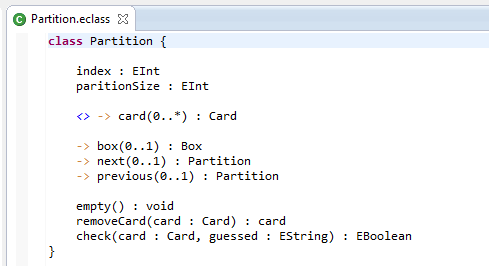
\includegraphics[width=0.6\textwidth]{eclipse_partitionMethods}
	\caption{The completed \texttt{Partition} EClass}
	\label{fig:partitionMethods}
\end{figure}

\vspace{0.5cm}

\item[$\blacktriangleright$] What needs to be done in the \texttt{Card} EClass? Well, in order to check the card, we'll need to be able to look at the flip
side. We'll also need to print whatever is on the current side. Create two paramater-less void functions, \texttt{invert} and \texttt{printCard}. 

\item[$\blacktriangleright$] Finally, what do we want to do with \texttt{Box}? In summary, we want a \texttt{Box} to:

\begin{description}
  \item[\texttt{determineNextSize():EInt}] Calculate how large a new partition in the box should be
  \item[\texttt{grow():void}] Increase the box by adding a new partition \update
  \item[\texttt{toString():EString}] Produce a string representation of the box with all its contents
  \item[\texttt{addToStringRep(card:Card):void}] Update the current string representation to include \texttt{card}
\end{description}

\item[$\blacktriangleright$] Implement the above signatures, and your entire workspace should now resemble Fig.~\ref{fig:workspaceMethods}.

\item[$\blacktriangleright$] Congratulations! You have now created a metamodel for our Learning Box using eMoflon's textual syntax! To see how
this looks in the visual syntax, check out Fig.~\ref{fig:metamodel_complete} from the previous section. As a final step, make sure you build the project and
wait for the package explorer to refresh. 

\newpage

\fancyfoot[R]{ $\triangleright$ \hyperlink{validation tex}{Next}}

\begin{figure}[htbp]
	\centering
  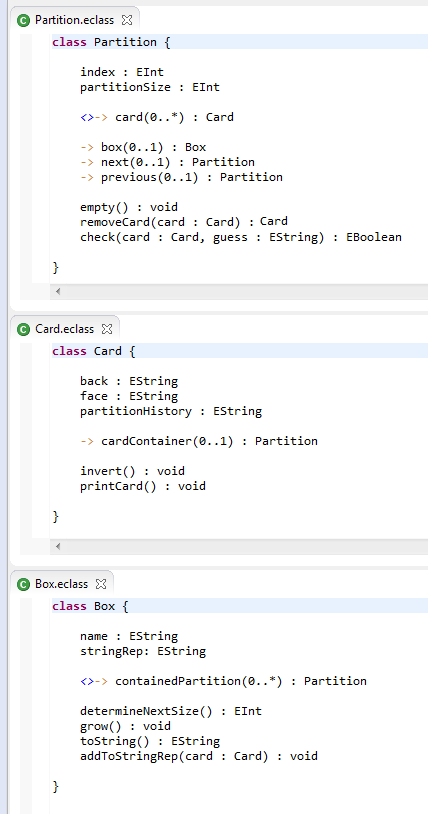
\includegraphics[width=0.7\textwidth]{eclipse_classesFullyDeclared}
	\caption{Completed method signatures}
	\label{fig:workspaceMethods}
\end{figure}
\FloatBarrier

\end{itemize}